\section{Bài 1: Ping}
Mở \textbf{\textit{ping.pcapng}} file, nội dung của file pcap là thông tin các gói tin gửi từ một máy sang một máy khác bằng lệnh ping.\\
Nội dung tập tin \textbf{\textit{ping.pcapng}} như sau.
\begin{figure}[H]
\begin{center}
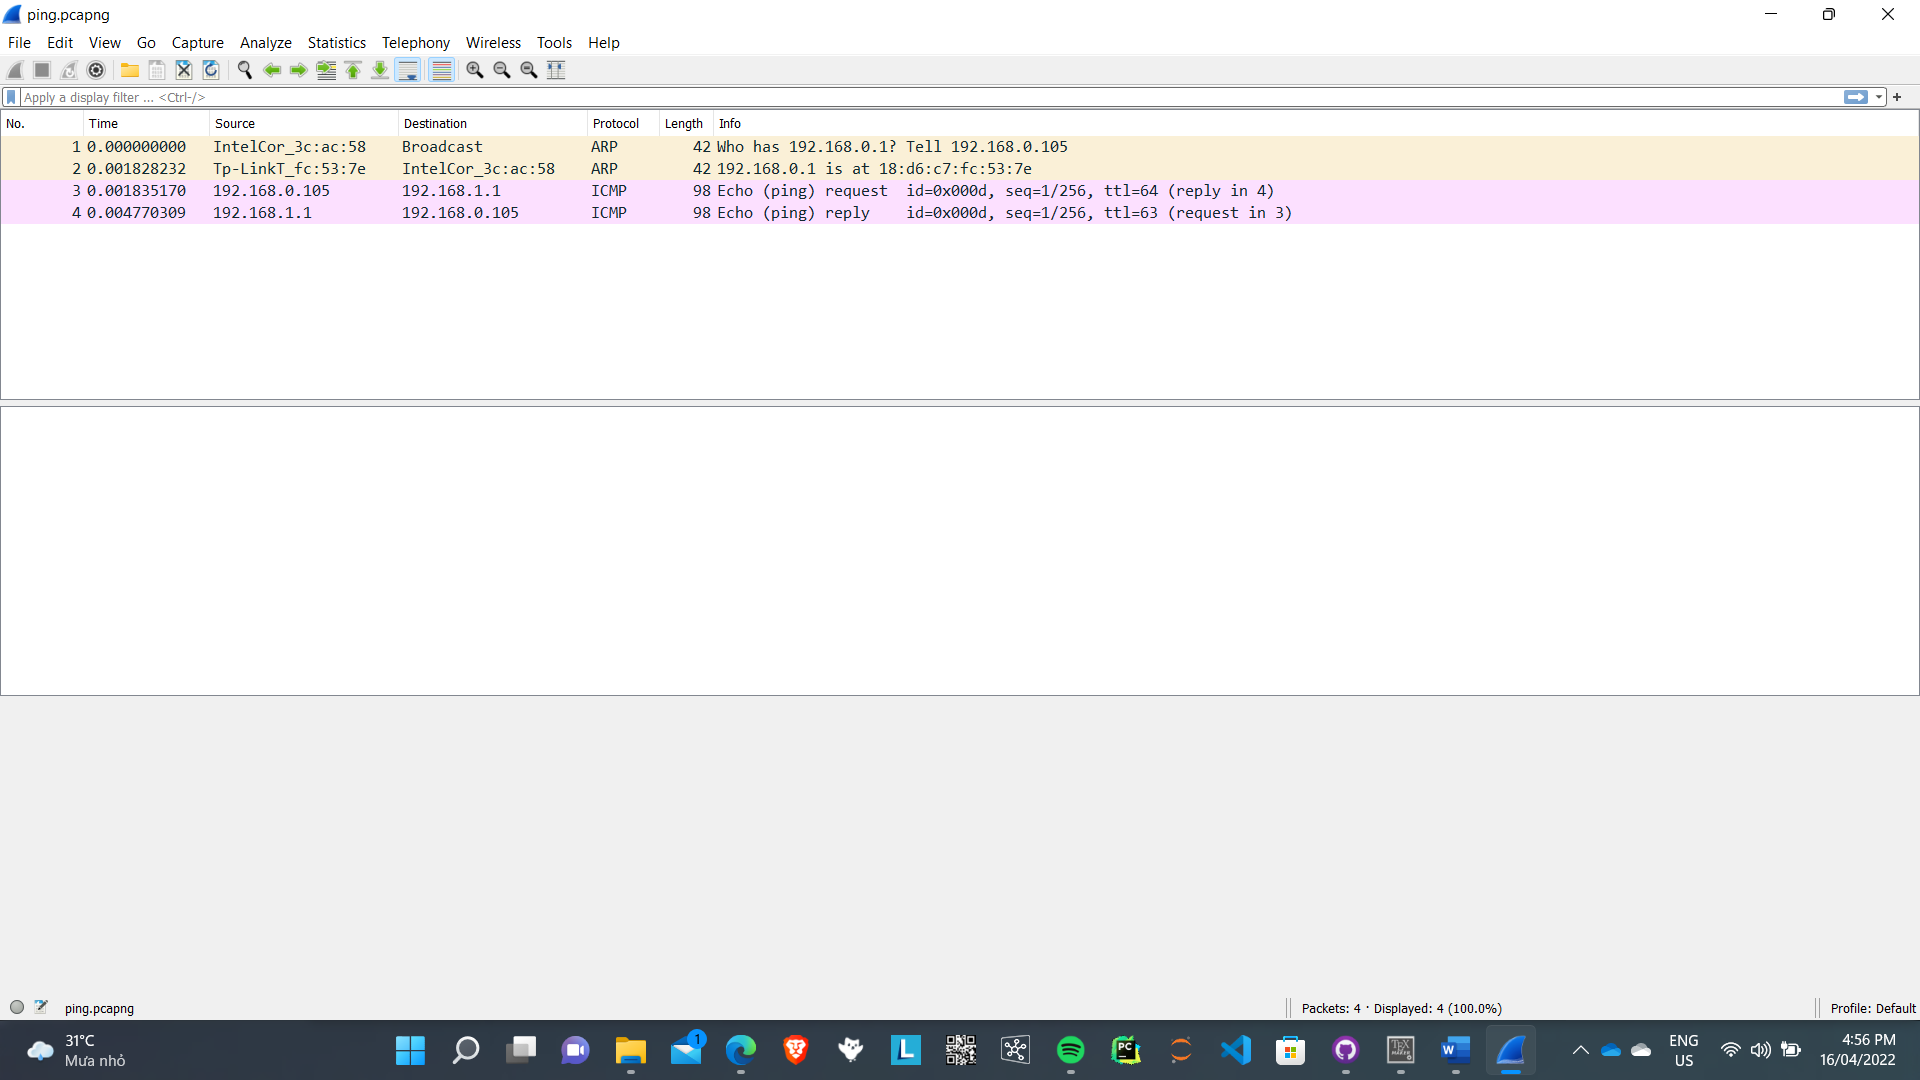
\includegraphics[scale=0.45]{../figures/p1/p1_ping}
\end{center}
\caption{Nội dung tập tin \textbf{\textit{ping.pcapng}}}
\end{figure}
Trả lời các câu hỏi sau:\\
\textbf{1.	Cho biết địa chỉ IP của host ping và host được ping?}\\
Địa chỉ IP của host ping: \textbf{192.168.0.105.}\\
Địa chỉ IP của host được ping: \textbf{192.168.1.1.}
\begin{figure}[H]
\begin{center}
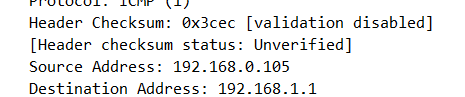
\includegraphics[scale=1]{../figures/p1/p1_r1}
\end{center}
\caption{Địa chỉ IP của host ping và host được ping}
\end{figure}

\textbf{2.	Cho biết port được sử dụng là bao nhiêu? Nếu không có port thì giải thích tại sao?}\\
\textbf{Không có} source port number và destination port number.\\
\textbf{Lý do:} Lệnh ping sử dụng giao thức \textbf{ICMP} của mô hình TCP/IP. ICMP là giao thức ở tầng, còn port number được sử dụng ở tầng Application.

\textbf{3.	Với gói tin ICMP request, cho biết kích thước (bytes) của từng phần trong diagram. (Chú ý: Kích thước tổng của gói tin là 98 bytes)}

\begin{table}[H]
\begin{center}
\begin{tabular}{|c|c|c|c|}
\hline 
ICMP data & ICMP header & IP header & Ethernet header \\ 
\hline 
48 & 16 & 20 & 14 \\ 
\hline 
\end{tabular} 
\end{center}
\caption{Kích thước gói tin ICMP request}
\end{table}

\begin{figure}[H]
\begin{center}
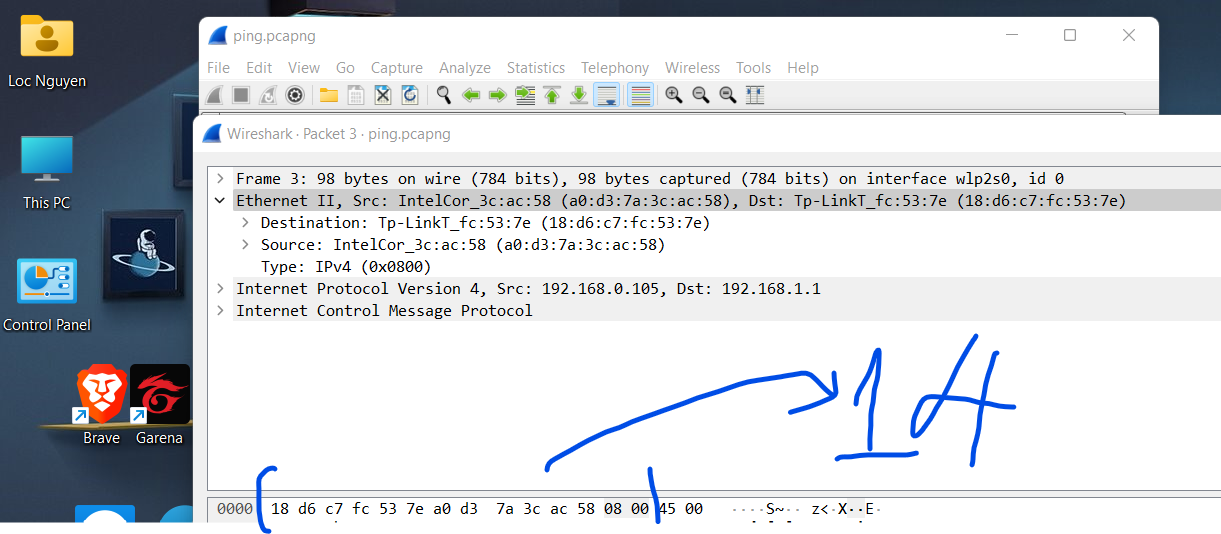
\includegraphics[scale=.8]{../figures/p1/p1_ethernet}
\end{center}
\caption{Độ dài Ethernet header}
\end{figure}

\begin{figure}[H]
\begin{center}
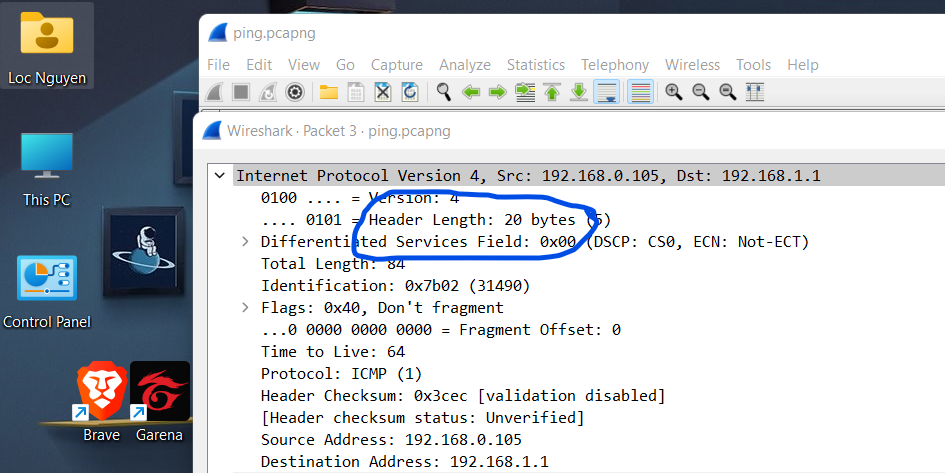
\includegraphics[scale=1]{../figures/p1/p1_ipheader}
\end{center}
\caption{Độ dài IP header}
\end{figure}

\begin{figure}[H]
\begin{center}
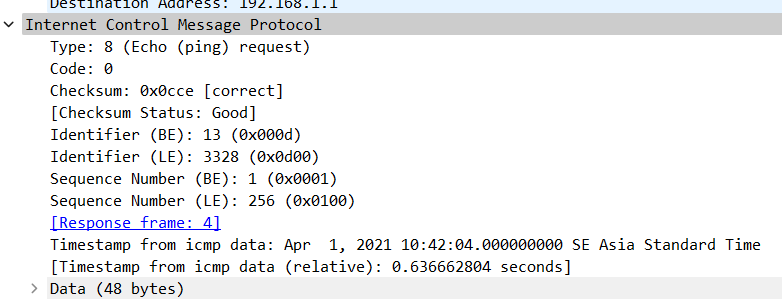
\includegraphics[scale=1]{../figures/p1/p1_icmp}
\end{center}
\caption{Độ dài ICMP data và ICMP header}
\end{figure}

\textbf{4.	Tại sao lại có 2 gói ARP?}\\
ARP (viết tắt của cụm từ Address Resolution Protocol) là giao thức mạng được dùng để tìm ra địa chỉ phần cứng (địa chỉ MAC) của thiết bị từ một địa chỉ IP nguồn. Nó được sử dụng khi một thiết bị giao tiếp với các thiết bị khác dựa trên nền tảng local network.\\
Khi ta sử dụng lệnh ping, host ping (192.168.0.105) thực hiện broadcast gói tin ARP request vào tất cả các host trong mạng LAN xem host nào có địa chỉ là 192.168.1.1 (host được ping). Host được ping sẽ gửi lại gói tin ARP reply, xác định địa chỉ MAC cần tìm (18:d6:c7:fc:53:7e) cho host ping.

\textbf{5.	Hãy vẽ sơ đồ mạng logic dựa trên nội dung gói pcap đó.} \\
Sơ đồ mạng logic dựa trên nội dung gói pcap trong bài như sau.
\begin{figure}[H]
\begin{center}
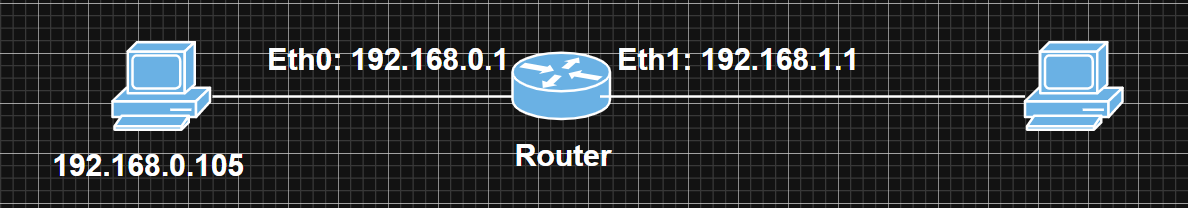
\includegraphics[scale=.75]{../figures/p1/p1_lan}
\end{center}
\caption{Sơ đồ mạng}
\end{figure}